\section{Data download and clustering analysis}

Price data on the ETFs is downloaded from Google Finance using the data download functionality built in to the Pandas module for Python.
We use the closing price of the ETF for each day to represent the day's price.
Any ETF with less than 2400 data points is excluded, leaving 93 of the initial 100 ETFs to use for further processing.

To cluster the data, it is necessary to define a distance between assets. We compute the correlation coefficient $C_{ij}$ between assets $i$ and $j$, and define the distance between them as
\begin{gather}
d(i,j) = 1 - C_{ij}^2  \in [0, 1].
\end{gather}
This distance will tend to group together assets that are more correlated and/or anti-correlated together.
This is intuitively a reasonable measure, as (1) going long on an asset is the same as going short on an asset that is anti-correlated with it, and we wish to treat short and long assets the same in this analysis, and (2) the difference between a correlation of 1.00 and 0.95 is more significant than between 0.05 and 0.00.


\begin{figure}[tp]
\centering
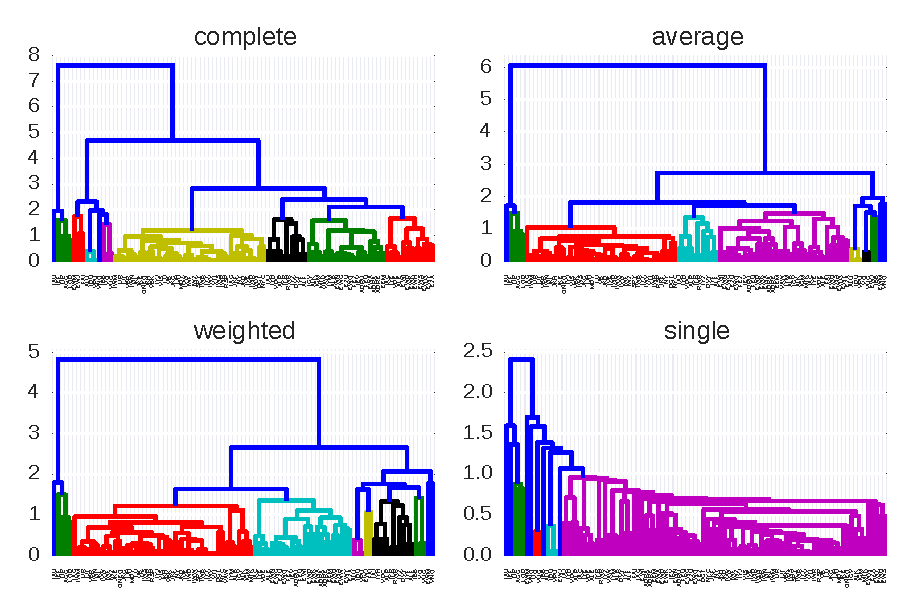
\includegraphics{pic/dendro_methods.pdf}
\caption{DELETE ME IN FINAL:\ Dendrogram of clustering found by various methods. All non-blue leaves are trimmed by the max-return and the min-std criteria.}
\label{fig:dendrogram}
\end{figure}

\begin{figure}[tp]
\centering
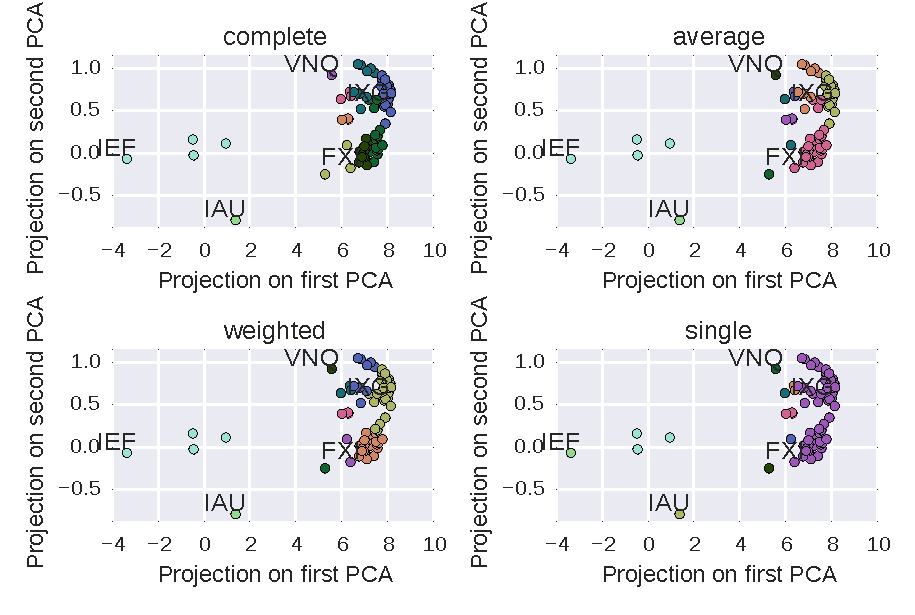
\includegraphics{pic/pca_methods.pdf}
\caption{Projection of asset correlation onto the largest principal components. These account for 78.58\% and 4.51\% of the variance, respectively.}
\label{fig:pca}
\end{figure}

\begin{figure}[tp]
\centering
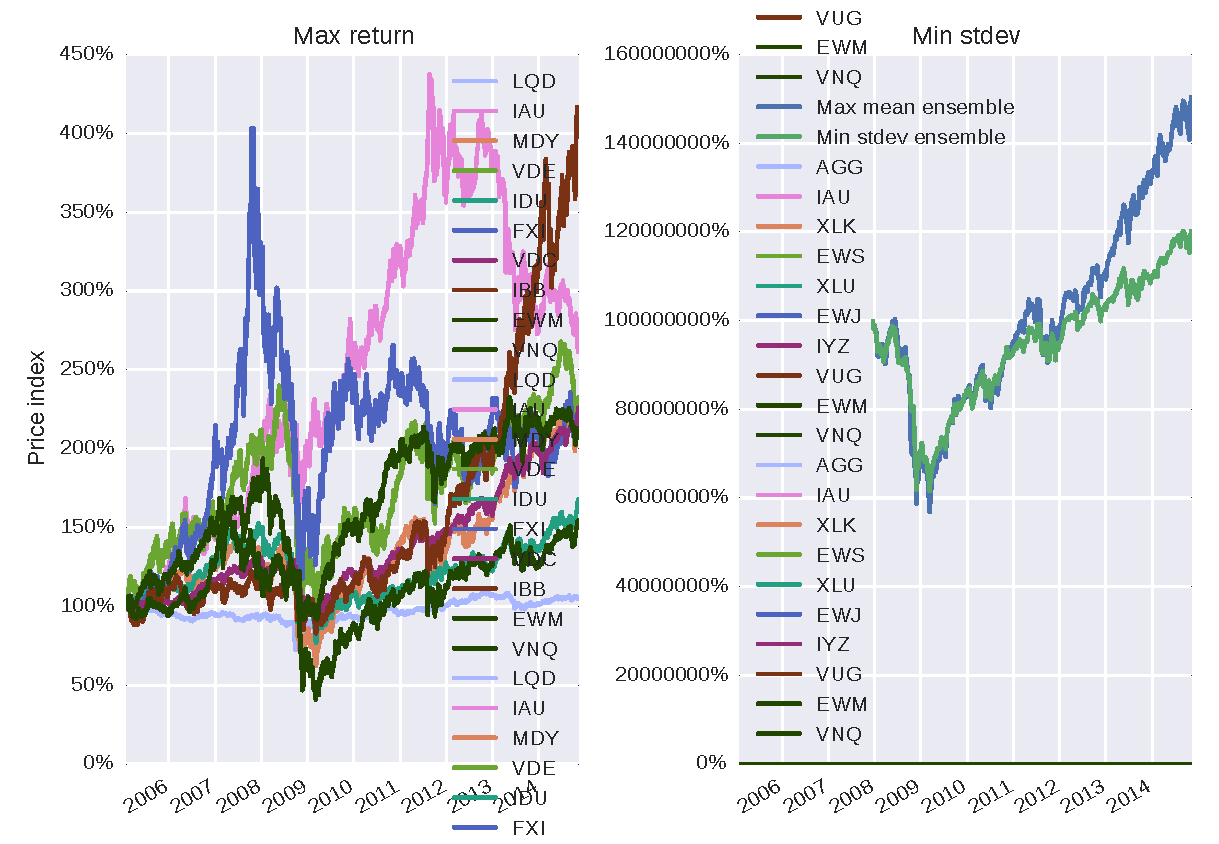
\includegraphics{pic/prices_selected_assets.pdf}
\caption{Price history for the assets selected by the max-return criteria (left) and the min-stdev criteria (right).}
\label{fig:prices_selected}
\end{figure}
